\documentclass[11pt]{article}
\usepackage[margin=1.15in]{geometry}
\usepackage{amsmath,amssymb,amsthm,stmaryrd}
\usepackage[expansion=false]{microtype}
\usepackage{booktabs}
\usepackage{enumitem}
\usepackage[T1]{fontenc}
\usepackage[hidelinks]{hyperref}
\usepackage{fancyvrb}
\usepackage{tikz}
\usetikzlibrary{arrows.meta,positioning,calc,fit}
\fvset{fontsize=\small,xleftmargin=1.5em}

\newtheorem{proposition}{Proposition}
\newtheorem{theorem}{Theorem}
\newtheorem{definition}{Definition}
\newtheorem{corollary}{Corollary}
\newcommand{\code}[1]{\texttt{#1}}
\newcommand{\cfg}[1]{\langle #1\rangle}
\newcommand{\step}{\longrightarrow}
\newcommand{\live}{\mathsf{live}}
\newcommand{\refuseval}{\mathsf{refuse}}
\newcommand{\faultval}{\mathsf{fault}}
\newcommand{\hash}{h}
\newcommand{\app}{\mathbin{\|}}
\newcommand{\pre}{\preceq}

\title{Following the Evaluator:\\An ASCII Language for Bounded State Transition}
\author{Flyxion\\Independent Researcher}
\date{September 2026}

\begin{document}
\maketitle

\begin{abstract}
Programming languages usually treat punctuation as a device for disambiguating parse trees. This essay develops the opposite discipline for a small symbolic language: every primitive symbol must correspond to a distinct restriction on the transitions the evaluator may perform. The starting point is the circles-of-evaluation notation used to teach nested expressions in Lisp-family languages. Extending the circle to a bounded region within which a proposed state transition is evaluated yields an ASCII language whose layout mirrors its execution structure. The essay separates concrete syntax, abstract syntax, and operational semantics, and proves a chain of properties for a deliberately small core calculus: unique parsing with canonical round trip, determinism, traversal decomposition, boundary locality with staged effects, legality of ledger histories with prefix extension, preservation of state under refusal and fault, verified commit, a two-directional correspondence between commits and valid witness records, threaded compositionality, and monotone narrowing under restrictive enclosing boundaries. These are combined in a single soundness theorem for bounded transitions. Beneath the proof chain lies a second chain of non-collapse principles, each instantiated in the calculus: representation is not referent, proposal is not realization, evaluation is not exposure, admission is not verification, event is not witness, refusal is not absence, persistence is not truth. Novelty is claimed only for the conjunction of individually familiar components.
\end{abstract}

\section{Introduction: From Notation to Motion}

In most languages a parenthesis is a grouping symbol. It resolves ambiguity in a string of tokens and then disappears into the syntax tree. In Lisp-family languages the parenthesis is the visible edge of a region of computation, and the nesting of parentheses is the nesting of evaluation. Teaching notations that draw expressions as nested circles make this explicit: to evaluate the outer circle, the evaluator first enters each inner circle, reduces it to a value, and hands that value outward.

That observation raises a design question narrower than the usual concerns of syntax design.

\begin{quote}
What would a programming language look like if its symbolic vocabulary were chosen according to restrictions on evaluator transitions rather than conventional syntactic categories?
\end{quote}

The answer developed here is a small language over printable ASCII. Its governing constraint is exclusionary: a symbol enters the language only if it corresponds to a restriction or operation on state transition that no other symbol already performs. The constraint prevents drift toward keyword-heavy syntax and keeps the relation between source text and execution checkable.

Every evocative sentence in the essay is meant to have a plain mathematical counterpart. Table~\ref{tab:pairs} collects the principal pairs. The geometric vocabulary of entering, following, and returning is an explanatory reading of a transition relation and not part of its definition. No claim is made that computation is spatial.

\begin{table}[h]
\centering
\small
\begin{tabular}{@{}p{0.44\linewidth}p{0.48\linewidth}@{}}
\toprule
Evocative statement & Formal counterpart \\
\midrule
Follow inward, return outward & Traversal decomposition (Prop.~\ref{p:trav}) and threaded compositionality (Prop.~\ref{p:comp}) \\
Entering a sphere is not committing & Boundary locality (Prop.~\ref{p:loc}) \\
No state change does not mean no event & $\Delta\sigma=0,\ \Delta\omega=0$ but $\lambda\pre\lambda'$ (Prop.~\ref{p:ref}) \\
Committed means verified and witnessed & Trace invariants (Props.~\ref{p:vc} and~\ref{p:corr}) \\
History cannot be rewritten & Prefix extension of the ledger (Prop.~\ref{p:legal}) \\
Return carrying only what every boundary admits & Restrictive operators narrow monotonically (Prop.~\ref{p:bound}) \\
The doorway, not the body & $r\neq x$ and $\mathrm{resolve}(r,\mathcal E)\rightharpoonup x$ (Section~\ref{s:door}) \\
\bottomrule
\end{tabular}
\caption{Metaphor and mathematics, paired.}
\label{tab:pairs}
\end{table}

The essay therefore has two spines. The first is a proof chain:
\begin{gather*}
\text{Parsing}\Rightarrow\text{Determinism}\Rightarrow\text{Staging isolation}\Rightarrow\text{Ledger legality}\\
\Rightarrow\text{Refusal and fault preservation}\Rightarrow\text{Commit soundness}\Rightarrow\text{Transaction soundness}.
\end{gather*}
The second is a family of non-collapse principles, collected in Section~\ref{s:noncollapse}, each of which is the statement that two objects ordinary description tends to identify are in fact distinct, and each of which is instantiated at a specific place in the first chain.

\section{Three Levels: Concrete Syntax, Abstract Syntax, Semantics}

Three objects are kept apart throughout:
\[
\text{ASCII source}\xrightarrow{\ \mathrm{parse}\ }\text{AST}\xrightarrow{\ \mathrm{evaluate}\ }\text{machine transitions}.
\]
The concrete syntax fixes which byte strings are programs. The abstract syntax fixes their structure. The operational semantics fixes what they do. The words ``sphere,'' ``enter,'' and ``return'' name readings of the third object and are not permitted to do work in the first two. A design that lets one level silently define another invites two kinds of objection: a reviewer may reject the formalization while accepting the idea, or a reader may take an illustration for a definition.

\begin{figure}[h]
\centering
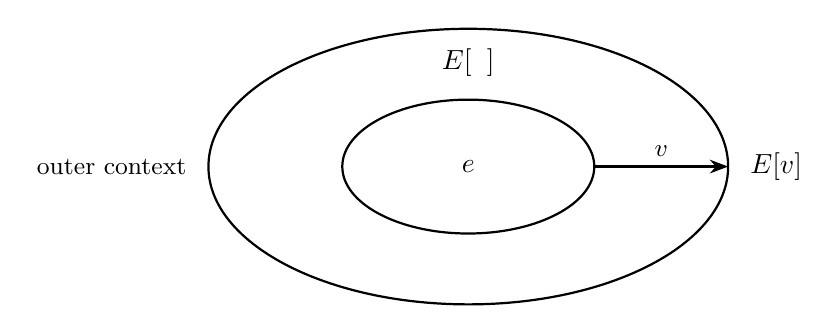
\begin{tikzpicture}[>=Stealth,thick,x=1cm,y=1cm]
\draw (0,0) ellipse (3.3 and 1.75);
\draw (0,0) ellipse (1.6 and 0.85);
\node at (0,1.32) {$E[\;\;]$};
\node at (0,0) {$e$};
\draw[->] (1.6,0) -- (3.3,0) node[midway,above] {\small $v$};
\node[right] at (3.45,0) {$E[v]$};
\node[left] at (-3.45,0) {\small outer context};
\end{tikzpicture}
\caption{Nested evaluation. The inner term $e$ is reduced under context $E$, and the value $v$ is returned to the context (Prop.~\ref{p:trav}). The figure depicts the decomposition of the transition relation and does not assert that evaluation moves through space.}
\end{figure}

\section{Design Principle: Motion Economy}

The alphabet is small. Table~\ref{tab:alpha} distinguishes symbols in the core calculus, for which proofs are given, from extensions specified only informally.

\begin{table}[h]
\centering
\small
\begin{tabular}{@{}clll@{}}
\toprule
Symbol & Motion & Status & Semantic role \\
\midrule
\code{( )} & enter, return & core & pure nested evaluation region \\
\code{<( )>} & open a bounded transition & core & delimits a frame with a staged store \\
\code{?} & admit & core & predicate on pre-state and proposal \\
\code{\~{}} & transform & core & pure change to the staged store \\
\code{!} & verify & core & predicate on the pair pre-state, staged result \\
\code{@} & attribute & core & construct provenance for the pending record \\
\code{>} & commit & core & atomically install the staged store and record \\
\code{\#} & persist & extension & flush the ledger to a durable host store \\
\code{\^{}} & reconstruct & extension & recovery from a recorded continuation \\
\code{|} & bind & extension & environment extension \\
\bottomrule
\end{tabular}
\caption{Alphabet and status.}
\label{tab:alpha}
\end{table}

\subsection{The admission rule and its two directions}

Let $\Sigma$ be the primitive symbols and $M$ the primitive evaluator motions, with $f:\Sigma\to M$ assigning each symbol its motion. The design principle has two halves.

\begin{quote}
\textbf{Economy.} $f$ is injective: $f(s_1)=f(s_2)\Rightarrow s_1=s_2$. No two primitive symbols denote the same motion.\\[2pt]
\textbf{Completeness.} For every motion $m$ in the declared core vocabulary $M_{\mathrm{core}}$ there is a symbol $s$ with $f(s)=m$.
\end{quote}
Together they push the core toward a bijection $\Sigma_{\mathrm{core}}\cong M_{\mathrm{core}}$. The distinction between the two halves matters: economy prevents redundancy, completeness prevents the silent use of unnamed motions. In the core of Table~\ref{tab:alpha}, the seven rows marked core form the seven motions, and the correspondence is checked by inspecting the transition rules of Section~\ref{s:core}: each rule belongs to exactly one motion, and each motion has at least one rule.

\subsection{The principle applied to its own notation}

The principle is useful only if it can reject the author's own choices. Three pressure tests are recorded.

\emph{Admission and verification.} If \code{?} and \code{!} were predicates over the same arguments they would be redundant. They are not. Admission reads only the committed store and the proposal, so it can be evaluated before any transformation has run. Verification reads the committed store, the staged store, and the pending effects together, so it can relate before and after. The two have different signatures, $\mathrm{Pred}(\sigma,v)$ and $\mathrm{Pred}(\sigma,\sigma^{\ast},\pi,v)$, and hence $\llbracket\,?\,\rrbracket\neq\llbracket\,!\,\rrbracket$ for a semantic reason. Stated abstractly:
\[
\text{admission is prospective; verification is relational.}
\]
Before an operation one asks whether it may begin given what is known. After transformation one asks whether the proposed before-and-after relation satisfies an invariant. These are different epistemic positions.

\emph{Attribution and persistence.} An earlier draft blurred \code{@} and \code{\#}. They are now separated: \code{@} constructs the provenance that will form part of the pending record, and \code{\#} is the flush of the ledger to a durable store. The first is a change to a frame, the second a change to the host. The ledger itself is appended at commit, discussed below.

\emph{Return and reconstruction.} An earlier draft assigned \code{\^{}} both to outward propagation and to reconstruction from a recorded continuation. Those are different motions and the assignment violated the principle. Return is performed by the closing delimiter \code{)}. The symbol \code{\^{}} is reserved for reconstruction and lives in the extensions. The commit symbol \code{>} likewise performs one motion, the atomic publication of a transition and its record. The atomicity is the point of the motion: the correspondence theorem of Section~\ref{s:corr} depends on the store change and the record being one step.

One token is reserved. Refusal is a result form written $\refuseval(t,r)$ in the semantics, and the bare identifier \code{x} is reserved in the concrete syntax for it. Such collisions are treated as costs of the constraint and not as grounds for relaxing it.

\section{The Core Calculus}\label{s:core}

\subsection{Abstract syntax}

Terms are
\[
\begin{array}{rcl}
e & ::= & a \;\mid\; (e_1\ \cdots\ e_n) \;\mid\; \langle\!(\,e\ ;\ c_1\cdots c_m\,)\!\rangle \\[2pt]
c & ::= & {?}\,p \;\mid\; {\sim}\,f \;\mid\; {!}\,q \;\mid\; {@}\,s \;\mid\; {>}\,g
\end{array}
\]
where $a$ ranges over atoms and $p,f,q,g$ over meta-level functions with the signatures below, drawn from a fixed signature environment:
\[
p:(\sigma,v)\rightharpoonup\{\top,\bot\},\quad
f:(\sigma^{\ast},v)\rightharpoonup(\sigma^{\ast},\pi,v),\quad
q:(\sigma,\sigma^{\ast},\pi,v)\rightharpoonup\{\top,\bot\},\quad
g:(\sigma^{\ast},v)\rightharpoonup v,
\]
with $\rightharpoonup$ marking partial functions whose undefinedness is a fault. The head expression $e$ of a bounded transition is the \emph{proposal}. It is evaluated to a value before the frame opens.

The commit function $g$ returns only a result value. It cannot supply a store. Commit installs the staged store $\sigma^{\ast}$, the store on which the verification predicates were evaluated, and never an independently supplied one. An earlier formulation in which the commit clause carried its own target state would have let a program manufacture a durable state unrelated to the verified one.

Runtime terms add the live frame
\[
\live(t,\,v,\,\sigma_0,\,\sigma^{\ast},\,\pi,\,A,\,\vec c),
\]
holding transition identifier $t$, proposal value $v$, snapshot $\sigma_0$ of the committed store, staged store $\sigma^{\ast}$, pending effects $\pi$, pending provenance $A$, and remaining clauses $\vec c$, together with the two non-committing results $\refuseval(t,r)$ and $\faultval(t)$. Equivalently, the machine executing inside a frame can be read as the five-tuple $\cfg{\vec c,\sigma,\sigma^{\ast},\lambda,\omega}$. The frame notation packages $\sigma^{\ast}$ and $\pi$ with the transition that owns them.

\subsection{Static semantics: well-formedness}

A bounded transition is well-formed only if its clause sequence matches
\[
{?}^{\ast}\ \ {\sim}^{\ast}\ \ {!}^{+}\ \ {@}^{+}\ \ {>}.
\]
That is: any number of admission tests, then any number of transformations, then at least one verification, then at least one attribution, then exactly one commit, last. The ordering is a static judgment and not an accident of grammar. Section~\ref{s:neg} shows what breaks when it is relaxed. Parsing is the partial function from ASCII source to well-formed ASTs.

\subsection{Configurations and outcomes}

The machine keeps four components apart,
\[
C=\cfg{e,\ \sigma,\ \lambda,\ \omega},
\]
where $\sigma$ is the committed program store, $\lambda\in\mathrm{Entry}^{\ast}$ is the ledger as a finite \emph{sequence}, and $\omega$ is the ordered trace of emitted external effects. Continuation is carried by the evaluation context in which the redex sits. Writing $\lambda\app\ell$ for appending an entry, and $\lambda\pre\lambda'$ for the prefix relation, the ledger is append-only in the strong sense that every later ledger has every earlier ledger as a prefix. Order matters: a set of entries cannot distinguish the history $\mathsf{adm},\mathsf{ver},\mathsf{wit}$ from the history $\mathsf{wit},\mathsf{adm},\mathsf{ver}$, and sequencing is what the legality theorem of Section~\ref{s:legal} constrains.

The outcome of a bounded transition is one of
\[
\mathrm{Outcome}\in\{\mathsf{commit},\ \mathsf{refuse},\ \mathsf{fault}\}.
\]
\emph{Refuse} means a predicate was evaluated and returned false. \emph{Fault} means evaluation could not be completed, for example because a predicate or transformer was undefined on its arguments, a store was unavailable, or a resource limit was reached. All three outcomes leave an entry in the ledger. The outcome of a run of a frame is the tag of the last rule applied to it.

\subsection{Evaluation contexts and reduction}

The places where reduction may occur are given by contexts,
\[
E ::= [\,]\ \mid\ (v_1\ \cdots\ v_{i-1}\ E\ e_{i+1}\cdots e_n)\ \mid\ \langle\!(\,E\ ;\ \vec c\,)\!\rangle,
\]
with the contextual rule
\[
\dfrac{\cfg{e,\sigma,\lambda,\omega}\step\cfg{e',\sigma',\lambda',\omega'}}
      {\cfg{E[e],\sigma,\lambda,\omega}\step\cfg{E[e'],\sigma',\lambda',\omega'}}
\]
and left-to-right call-by-value order. A pure application whose arguments are values reduces by a primitive function table $\delta$. A fault propagates: $E[\faultval(t)]\step\faultval(t)$ for $E\neq[\,]$. A refusal is an ordinary value and propagates as data.

The rules for bounded transitions follow. Throughout, $\sigma_0,\sigma^{\ast},\pi,A,v,t$ are the live frame's components.

\medskip
\noindent\textbf{Open.} With $t$ fresh (one more than the number of \textsf{open} entries in $\lambda$) and $Q$ the set of verification clauses of the transition:
\[
\cfg{\langle\!(v;\vec c)\!\rangle,\sigma,\lambda,\omega}\step
\cfg{\live(t,v,\sigma,\sigma,\varepsilon,\varnothing,\vec c),\ \sigma,\ \lambda\app\mathsf{open}(t,\hash(\sigma),Q),\ \omega}.
\]
\noindent\textbf{Admit.} Let $p(\sigma_0,v)$ be the predicate value.
\[
\begin{array}{ll}
p(\sigma_0,v)=\top: & \live(\ldots,({?}p)\!::\!\vec c)\step\live(\ldots,\vec c),\ \ \lambda\app\mathsf{adm}(t,p)\\
p(\sigma_0,v)=\bot: & \live(\ldots,({?}p)\!::\!\vec c)\step\refuseval(t,{?}p),\ \ \lambda\app\mathsf{ref}(t,{?}p)\\
p(\sigma_0,v)\ \text{undefined}: & \live(\ldots,({?}p)\!::\!\vec c)\step\faultval(t),\ \ \lambda\app\mathsf{flt}(t,{?}p)
\end{array}
\]
\noindent\textbf{Transform.} If $f(\sigma^{\ast},v)=(\sigma^{\ast\prime},\pi',v')$ then
\[
\live(t,v,\sigma_0,\sigma^{\ast},\pi,A,({\sim}f)\!::\!\vec c)\step\live(t,v',\sigma_0,\sigma^{\ast\prime},\pi\cdot\pi',A,\vec c),
\]
with $\sigma$, $\lambda$, and $\omega$ untouched. The rule changes the staged store and the pending effects and nothing else. If $f$ is undefined the frame faults with $\mathsf{flt}(t,{\sim}f)$.

\noindent\textbf{Verify.} With $q(\sigma_0,\sigma^{\ast},\pi,v)$: on $\top$ the frame advances and $\lambda\app\mathsf{ver}(t,q)$; on $\bot$ it reduces to $\refuseval(t,{!}q)$ with $\lambda\app\mathsf{ref}(t,{!}q)$; if undefined it faults with $\mathsf{flt}(t,{!}q)$.

\noindent\textbf{Attribute.} $\live(\ldots,A,({@}s)\!::\!\vec c)\step\live(\ldots,A\cup\{s\},\vec c)$. The provenance is not yet in the ledger. It becomes part of the single record produced at commit.

\noindent\textbf{Commit.} Let $V=\{q\mid \mathsf{ver}(t,q)\text{ occurs in }\lambda\}$ and $w=\langle t,\hash(\sigma_0),\hash(\sigma^{\ast}),V,A\rangle$. Then
\[
\cfg{\live(t,v,\sigma_0,\sigma^{\ast},\pi,A,[{>}g]),\ \sigma,\ \lambda,\ \omega}\step
\cfg{g(\sigma^{\ast},v),\ \sigma^{\ast},\ \lambda\app\mathsf{wit}(w),\ \omega\cdot\pi}.
\]
The commit rule is the only rule that changes $\sigma$ or $\omega$. It installs the verified staged store, emits the pending effects, and appends exactly one witness record, in one step. If $g$ is undefined the frame faults and nothing is installed.

\section{Parsing, Determinism, and Traversal}

\begin{proposition}[Unique parsing and canonical round trip]\label{p:parse}
Let $\mathrm{print}$ be the canonical printer from well-formed ASTs to ASCII. Then $\mathrm{parse}(\mathrm{print}(a))=a$ for every well-formed $a$, and $\mathrm{print}(\mathrm{parse}(s))=s$ for every canonical source $s$. Consequently, for every parsable $s$,
\[\mathrm{parse}(\mathrm{print}(\mathrm{parse}(s)))=\mathrm{parse}(s).\]
\end{proposition}
\begin{proof}
The delimiters \code{(} and \code{<(} are distinct tokens, each clause symbol is a single reserved character, and atoms are maximal runs of non-reserved, non-whitespace characters. The grammar is therefore uniquely readable by one-token lookahead, so the parse tree of a source is unique. The printer emits tokens in tree order with fixed spacing and indentation, and reading that output recovers the same tree. The second and third statements follow by composition.
\end{proof}

\begin{proposition}[Determinism]\label{p:det}
If the meta-level functions $p,f,q,g,\delta$ are deterministic, then $C\step C_1$ and $C\step C_2$ imply $C_1=C_2$.
\end{proposition}
\begin{proof}
Every term other than a value decomposes uniquely as $E[r]$ for a redex $r$, by the left-to-right definition of contexts. Redexes are distinguished by their head form, and a live frame by the kind of its first remaining clause and by the value of the deciding predicate, so at most one rule applies. The fresh identifier is a function of $\lambda$. Hence the successor is unique.
\end{proof}

Determinism is a property of the core. Interleaving, external resources, and unavailable stores would each introduce named sources of nondeterminism, identified when they are added.

\begin{proposition}[Traversal decomposition]\label{p:trav}
Let $e$ not be a value and let $E$ be an evaluation context.
\begin{enumerate}[label=(\alph*)]
\item If $\cfg{e,\sigma,\lambda,\omega}\step^{\ast}\cfg{v,\sigma',\lambda',\omega'}$ then $\cfg{E[e],\sigma,\lambda,\omega}\step^{\ast}\cfg{E[v],\sigma',\lambda',\omega'}$.
\item Conversely, in any run of $E[e]$ the first steps are steps of $e$ under $E$, until $e$ is a value or faults, and the run factors through $E[v]$ for that value $v$.
\end{enumerate}
\end{proposition}
\begin{proof}
(a) follows from the contextual rule by induction on the length of the run of $e$. For (b), while $e$ is not a value it contains the leftmost redex of $E[e]$, since $E$ consists of values to the left of the hole. By Proposition~\ref{p:det} no other step is available. If $e$ faults, the fault rule collapses $E[\faultval(t)]$ to $\faultval(t)$. Otherwise the run reaches $E[v]$.
\end{proof}

This is the exact content of ``follow inward, return outward.'' The traversal of a nested term factors, as a matter of the transition relation, into an inner run followed by an outer run.

\begin{proposition}[Threaded compositionality]\label{p:comp}
Write $S=(\sigma,\lambda,\omega)$ and $\langle e,S\rangle\Downarrow\langle v,S'\rangle$ for $\langle e,S\rangle\step^{\ast}\langle v,S'\rangle$. Then
\[
\dfrac{\langle e,S\rangle\Downarrow\langle v,S'\rangle\qquad\langle E[v],S'\rangle\Downarrow\langle r,S''\rangle}
      {\langle E[e],S\rangle\Downarrow\langle r,S''\rangle}.
\]
Moreover, if $e$ is \emph{pure}, meaning that its run leaves $\sigma$, $\lambda$, $\omega$ unchanged, then $E[e]\approx E[v]$, where the observer sees the final value together with $\sigma$, $\lambda$, and $\omega$. If $e$ is not pure, then $E[e]$ is observationally equivalent to $E[v]$ run from $S'$, and not to $E[v]$ run from $S$.
\end{proposition}
\begin{proof}
The rule is Proposition~\ref{p:trav}(a) followed by the second premise. For a pure $e$, $S'=S$, so the two runs coincide. For a non-pure $e$ the two runs differ in starting store, ledger, or effect trace, and the observer can see all three.
\end{proof}

The qualification matters. The naive statement $C[e]\equiv C[v]$ fails as soon as $e$ has an effect on the ledger.

\section{Staging: Locality, Exposure, and Isolation}

\begin{proposition}[Boundary locality]\label{p:loc}
Between the open step and the commit step of a bounded transition, the committed store $\sigma$ and the effect trace $\omega$ are equal to their values at the open step.
\end{proposition}
\begin{proof}
By inspection of the rules applicable to a live frame: admit, transform, verify, and attribute read $\sigma_0$ and modify only the frame components $\sigma^{\ast}$, $\pi$, $A$ and the ledger. Only the commit rule writes $\sigma$ or $\omega$. Because the core is sequential and reduction is deterministic, no other redex runs while the frame is live.
\end{proof}

Entering a sphere is not equivalent to committing its intermediate states. The result depends on the design and not on the notation: it holds because $\sim$ acts on a staged store and returns proposed effects, and not because transformations are written inside delimiters. Abstractly,
\[
\text{evaluation need not imply exposure:}\qquad \mathrm{computed}(x)\not\Rightarrow\mathrm{exposed}(x).
\]
Intermediate computation can occur while durable state and external effects remain unchanged, and commit is the operation that converts a private, provisional consequence into a public, durable one. The pattern is familiar from databases, simulation, publishing, and review processes. Figure~\ref{f:annulus} shows it.

\begin{figure}[h]
\centering
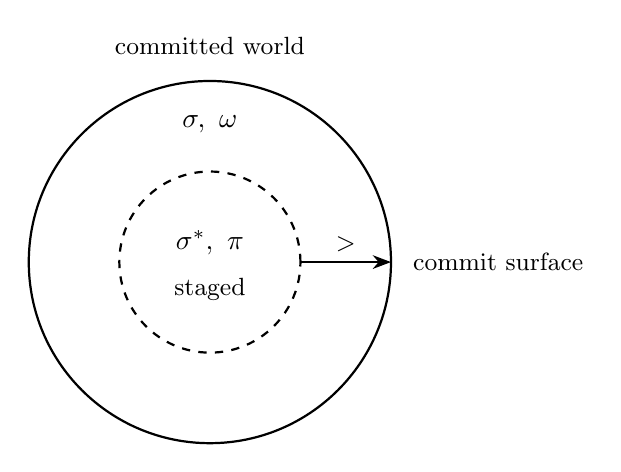
\begin{tikzpicture}[>=Stealth,thick]
\draw (0,0) circle (2.3);
\draw[dashed] (0,0) circle (1.15);
\node at (0,0.25) {$\sigma^{\ast},\ \pi$};
\node at (0,-0.35) {\small staged};
\node at (0,1.75) {$\sigma,\ \omega$};
\node at (0,2.75) {\small committed world};
\draw[->] (1.15,0) -- (2.3,0) node[midway,above] {\small $>$};
\node[right] at (2.45,0) {\small commit surface};
\end{tikzpicture}
\caption{Boundary locality. The interior may change while the exterior does not: $\sigma^{\ast}_{t+1}\neq\sigma^{\ast}_t$ while $\sigma_{t+1}=\sigma_t$. Only crossing the commit surface permits $\sigma\leftarrow\sigma^{\ast}$ and $\omega\leftarrow\omega\cdot\pi$.}
\label{f:annulus}
\end{figure}

\paragraph{Rollback versus isolation.} If a transformation could perform an irreversible external effect, for instance send a packet or actuate hardware, then
\begin{Verbatim}
~ transform
! verify
> commit
\end{Verbatim}
would not provide the bounded behaviour the notation suggests, because a later refusal could not undo an earlier effect. The core rules out this case by typing: $f$ returns \emph{proposed} effects, and $\omega$ is written only at commit. An extension that permits effects classified as compensable, reversible, or irrevocable must say which class may occur before verification. The conservative rule is that only staged or compensable effects may precede it, and irrevocable effects may occur only through the commit clause.

\paragraph{Which guarantees are claimed.} The word ``transaction'' brings database expectations. The core provides atomicity of the change to $(\sigma,\omega)$, in the sense that both change together at one step or not at all, and a form of consistency, in the sense that verification predicates hold on the staged result at commit. Isolation is trivial in a sequential core and would need a validation step under concurrency. Durability is not provided by the core and belongs to the flush motion \code{\#}. For these reasons the essay uses \emph{bounded transition} and reserves \emph{transaction} for statements limited to these properties.

\section{Ledger Legality, Refusal, and Fault}\label{s:legal}

Prefix extension says only that history is not rewritten. A stronger property is that only legal histories can be written at all. Each bounded transition, viewed through the ledger, follows a small protocol, shown in Figure~\ref{f:proto}.

\begin{figure}[h]
\centering
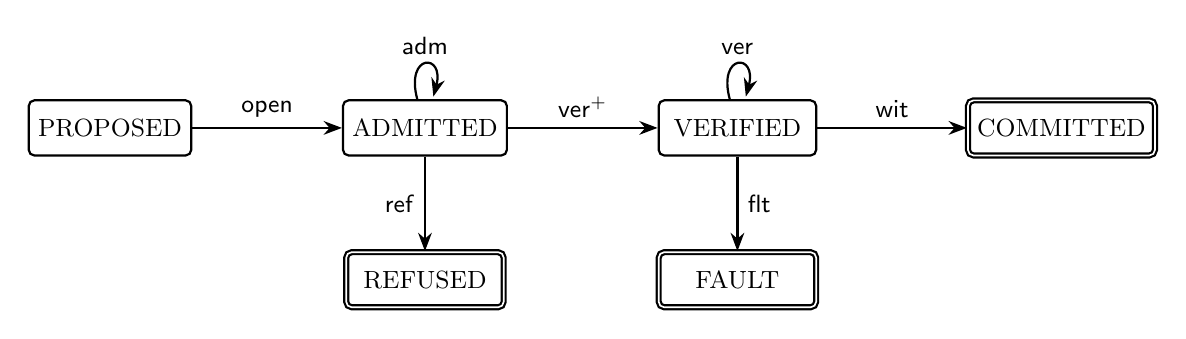
\begin{tikzpicture}[>=Stealth,thick,node distance=1.6cm and 1.9cm,
  st/.style={draw,rounded corners=2pt,minimum width=2.0cm,minimum height=0.7cm,font=\small},
  end/.style={draw,double,rounded corners=2pt,minimum width=2.0cm,minimum height=0.7cm,font=\small}]
\node[st] (op) {PROPOSED};
\node[st,right=of op] (ad) {ADMITTED};
\node[st,right=of ad] (ve) {VERIFIED};
\node[end,right=of ve] (co) {COMMITTED};
\node[end,below=1.2cm of ad] (re) {REFUSED};
\node[end,below=1.2cm of ve] (fa) {FAULT};
\draw[->] (op) -- node[above]{\small $\mathsf{open}$} (ad);
\draw[->] (ad) -- node[above]{\small $\mathsf{ver}^{+}$} (ve);
\draw[->] (ve) -- node[above]{\small $\mathsf{wit}$} (co);
\draw[->] (ad) -- node[left]{\small $\mathsf{ref}$} (re);
\draw[->] (ve) -- node[right]{\small $\mathsf{flt}$} (fa);
\draw[->] (ad) edge[loop above] node[above]{\small $\mathsf{adm}$} (ad);
\draw[->] (ve) edge[loop above] node[above]{\small $\mathsf{ver}$} (ve);
\end{tikzpicture}
\caption{The per-transition ledger protocol. Refusal and fault are reachable from admitted and verified states alike. The diagram abbreviates the regular language $\mathcal L_t$ of Proposition~\ref{p:legal}.}
\label{f:proto}
\end{figure}

Let $\mathcal L_t$ be the set of words over ledger entries tagged with identifier $t$ given by
\[
\mathsf{open}\ \mathsf{adm}^{\ast}\ \mathsf{ver}^{\ast}\ (\mathsf{ref}\mid\mathsf{flt})\ \ \big|\ \ \mathsf{open}\ \mathsf{adm}^{\ast}\ \mathsf{ver}^{+}\ \mathsf{wit}.
\]

\begin{proposition}[Ledger legality and prefix extension]\label{p:legal}
Let $\lambda_0=[\,]$ and let $\lambda$ be the ledger at any point of a run. Then
\begin{enumerate}[label=(\alph*)]
\item for every step $C\step C'$, $\lambda\pre\lambda'$;
\item $\lambda$ is a prefix of a concatenation $w_1w_2\cdots w_k$ with each $w_i\in\mathcal L_{t_i}$, in order of opening;
\item every frame that opens terminates in exactly one of \textsf{commit}, \textsf{refuse}, \textsf{fault} after at most $m+1$ steps, where $m$ is its clause count.
\end{enumerate}
\end{proposition}
\begin{proof}
(a) Every rule either leaves $\lambda$ unchanged or appends. (b) is by induction on the number of steps. A frame is created by the open rule, which appends $\mathsf{open}$. Each clause rule appends the entry its clause kind licenses: \textsf{adm} only from an admission clause, \textsf{ver} only from a verification clause. By well-formedness, admission clauses precede verification clauses, so entries appear in the order of the regular expression. A frame ends only with a \textsf{ref}, \textsf{flt}, or \textsf{wit}, after which no further entry carries its identifier. Because the core is sequential, each frame runs to completion before another opens, so the words for distinct transitions do not interleave. (c) Each clause rule consumes one clause and leads to a further frame, a refuse or fault value, or, for the last clause, the commit rule. The commit rule is defined only for the single remaining clause, which well-formedness guarantees is $>g$.
\end{proof}

The proposition says something stronger than that history persists. Illegal histories cannot be generated by the semantics. The ledger cannot contain a witness before a verification, a witness after a refusal, or two witnesses for one transition, whatever the program.

\begin{proposition}[Refusal and fault preservation]\label{p:ref}
Suppose a bounded transition opened in $(\sigma,\lambda,\omega)$ reduces to $\refuseval(t,r)$ or to $\faultval(t)$ with final components $(\sigma',\lambda',\omega')$. Then $\sigma'=\sigma$, $\omega'=\omega$, and $\lambda\pre\lambda'$, with $\lambda'=\lambda\app w$ for some $w\in\mathcal L_t$ ending in $\mathsf{ref}$ or $\mathsf{flt}$.
\end{proposition}
\begin{proof}
By Proposition~\ref{p:loc} the store and effect trace are unchanged until commit, and the refuse and fault rules are reached only from a live frame before the commit clause. The ledger difference is given by Proposition~\ref{p:legal}(b).
\end{proof}

Hence
\[
\mathrm{REFUSE}(e)\ \Rightarrow\ \Delta\sigma=0\ \land\ \Delta\omega=0,\qquad\text{while }\Delta\lambda\neq 0.
\]
No state change does not imply that no event occurred. Writing $I$ for information about an attempted transition, $\Delta\sigma=0\not\Rightarrow\Delta I=0$. A refused proposal leaves the world unchanged and leaves evidence that it was evaluated. Negative events are events: the three-way outcome makes all of \textsf{commit}, \textsf{refuse}, and \textsf{fault} part of the history of evaluation, and the ledger tags refusal and fault differently, so that a timeout, a malformed transformer, or an unavailable store is not confused with a decision.

\subsection{Proposal, evaluation, realization}

The results above prove that three notions ordinary description merges are distinct. Let $\mathcal P$ be the proposals made, $\mathcal E$ those evaluated, and $\mathcal R$ those realized in the committed store. Then $\mathcal R\subseteq\mathcal E\subseteq\mathcal P$, and refusal and fault occupy $\mathcal E\setminus\mathcal R$ (Figure~\ref{f:pre}). A proposal can exist without being evaluated, can be evaluated without being realized, and can leave evidence of evaluation without becoming state. The category error avoided is the treatment of the representation of a possibility as the execution of that possibility.

\begin{figure}[h]
\centering
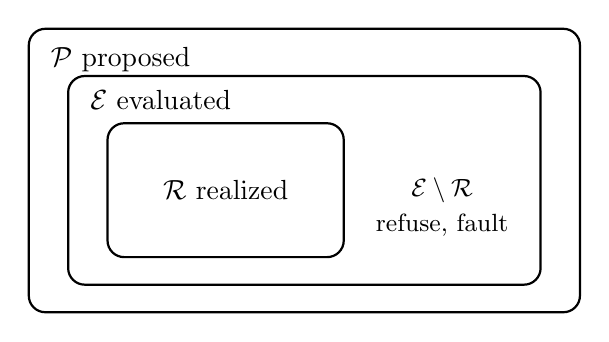
\begin{tikzpicture}[thick]
\draw[rounded corners=6pt] (0,0) rectangle (7,3.6);
\draw[rounded corners=6pt] (0.5,0.35) rectangle (6.5,3.0);
\draw[rounded corners=6pt] (1.0,0.7) rectangle (4.0,2.4);
\node[anchor=north west] at (0.15,3.5) {$\mathcal P$ proposed};
\node[anchor=north west] at (0.65,2.95) {$\mathcal E$ evaluated};
\node at (2.5,1.55) {$\mathcal R$ realized};
\node at (5.25,1.55) {\small $\mathcal E\setminus\mathcal R$};
\node at (5.25,1.1) {\small refuse, fault};
\end{tikzpicture}
\caption{Proposal, evaluation, realization. Refusal and fault are evaluated but not realized.}
\label{f:pre}
\end{figure}

\subsection{Non-retroactivity}

Refusal is terminal in a precise sense. By Proposition~\ref{p:legal}(a) the entry $\mathsf{ref}(t,\cdot)$, once appended, is in every later ledger, and the only rule that appends $\mathsf{wit}$ for $t$ is the commit rule applied to the frame of $t$, which no longer exists. No rule takes $\refuseval(t,r)$ as input and produces a commit. An enclosing context may inspect the value as data, react to it, and run a fresh bounded transition, and it may not make the historical claim that $t$ committed true. Generalized:
\[
\text{a later context may reinterpret an outcome but cannot rewrite its occurrence.}
\]

\section{Verified Commit and Witness Correspondence}\label{s:corr}

\subsection{Recorded versus valid}

Presence of a ledger entry is not evidence that its content is correct. A witness is \emph{recorded} when it occurs in $\lambda$. It is \emph{valid} with respect to a trace prefix $\rho$ when it satisfies conditions that can be checked against the trace independently of the commit rule.

\begin{definition}[Valid witness]
$\mathrm{ValidWitness}(w,\rho)$ holds when $w=\langle t,a,b,V,A\rangle$ and in $\rho$: there is a unique $\mathsf{open}(t,a',Q)$ with $a=a'$; the committed store immediately before $t$'s commit step has hash $a$; the committed store immediately after has hash $b$; $Q\subseteq V$; and $A\neq\varnothing$.
\end{definition}

The hash function is assumed injective on reachable stores (Assumption~H). This is a modelling assumption that lets hash equality stand for store equality and is not a cryptographic claim.

\subsection{Verified commit}

\begin{proposition}[Verified commit]\label{p:vc}
Let $\rho$ be any run of a program whose bounded transitions are well-formed. If a commit step for transition $t$ occurs in $\rho$, then before that step the ledger contains $\mathsf{ver}(t,q)$ for every $q\in Q_t$, contains no $\mathsf{ref}(t,\cdot)$ or $\mathsf{flt}(t,\cdot)$, and $A_t\neq\varnothing$.
\end{proposition}
\begin{proof}
The clause sequence is consumed head first. By well-formedness the commit clause is last, so the frame reaches $[{>}g]$ only after every earlier clause has been consumed. A verification clause is consumed only by the verify-true rule, which appends $\mathsf{ver}(t,q)$. A refusal or fault ends the frame and no later clause is reached. Well-formedness requires at least one attribution clause, and each such clause adds to $A$.
\end{proof}

The result follows from the interaction between the static ordering discipline and the small-step rules. It is not a definitional tautology, since it fails for programs that are not well-formed (Section~\ref{s:neg}).

\subsection{Correspondence}

\begin{proposition}[Witness correspondence]\label{p:corr}
For every run $\rho$ from an initial configuration with empty ledger and every prefix of it:
\begin{enumerate}[label=(\alph*)]
\item every step that changes $\sigma$ or $\omega$ is a commit step;
\item every commit step appends exactly one \textsf{wit} entry, and that entry is valid with respect to the prefix ending at that step;
\item every \textsf{wit} entry in the ledger arises from exactly one commit step.
\end{enumerate}
Consequently the number of commit steps equals the number of valid witness records in the ledger, at every prefix.
\end{proposition}
\begin{proof}
(a) is established by inspecting the rules: only commit writes $\sigma$ or $\omega$. For (b), the commit rule appends one record. Its \textsf{open} entry exists because the frame was created by the open rule, its pre-hash equals $\hash(\sigma_0)$ and, by Proposition~\ref{p:loc}, $\sigma_0$ equals the committed store immediately before the commit step. Its post-hash is $\hash(\sigma^{\ast})$, the store installed by the step. The verified set $V$ is read from the ledger and contains $Q_t$ by Proposition~\ref{p:vc}. For (c), no rule other than commit appends a \textsf{wit} entry.
\end{proof}

The correspondence gives what may be called conservation of committed history:
\[
\#\mathrm{Commit}=\#\mathrm{ValidWitness}.
\]
It is stronger than ordinary auditability. Auditability asserts $\mathrm{Commit}\to\mathrm{Witness}$. The invariant here is $\mathrm{Commit}\leftrightarrow\mathrm{ValidWitness}$: committed change cannot appear without a corresponding witness record, and records of that class cannot appear without committed change. Part (a) catches back doors. Parts (b) and (c) give the converse. Figure~\ref{f:bip} shows the matching and its failure modes.

\begin{figure}[h]
\centering
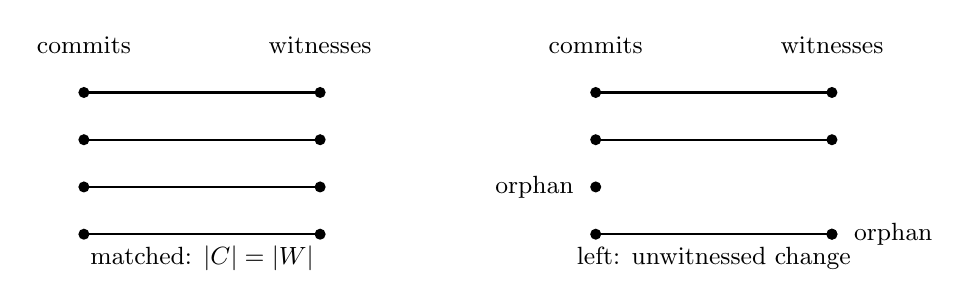
\begin{tikzpicture}[thick,every node/.style={font=\small}]
\begin{scope}
\node at (0,2.3) {commits};
\node at (3,2.3) {witnesses};
\foreach \i in {1,...,4}{
  \fill (0,2.3-0.6*\i) circle (2pt);
  \fill (3,2.3-0.6*\i) circle (2pt);
  \draw (0,2.3-0.6*\i) -- (3,2.3-0.6*\i);
}
\node at (1.5,-0.4) {matched: $|C|=|W|$};
\end{scope}
\begin{scope}[xshift=6.5cm]
\node at (0,2.3) {commits};
\node at (3,2.3) {witnesses};
\foreach \i in {1,2,4}{
  \fill (0,2.3-0.6*\i) circle (2pt);
  \draw (0,2.3-0.6*\i) -- (3,2.3-0.6*\i);
  \fill (3,2.3-0.6*\i) circle (2pt);
}
\fill (0,2.3-1.8) circle (2pt);
\fill (3,2.3-2.4) circle (2pt);
\node[left] at (-0.15,2.3-1.8) {orphan};
\node[right] at (3.15,2.3-2.4) {orphan};
\node at (1.5,-0.4) {left: unwitnessed change};
\end{scope}
\end{tikzpicture}
\caption{Commit and witness correspondence (Prop.~\ref{p:corr}). In the right panel, a left orphan is a state change without a witness and a right orphan is a witness without a state change. Both are excluded.}
\label{f:bip}
\end{figure}

\subsection{Event and witness}

A witness relates the endpoints of a transition and is not the transition. Figure~\ref{f:chord} shows the relation, and the record is $w=\langle t,\hash(\sigma_0),\hash(\sigma_1),V,A\rangle$. Yet the record can constrain later events, and Section~\ref{s:prin} returns to that.

\begin{figure}[h]
\centering
\begin{tikzpicture}[>=Stealth,thick]
\node (a) at (0,0) {$\sigma_0$};
\node (b) at (5,0) {$\sigma_1$};
\draw[->] (a) -- node[below]{$T$} (b);
\draw[->,dashed] (a) to[bend left=60] node[above]{$w$} (b);
\end{tikzpicture}
\caption{A witness relates the endpoints of a transition ($w\neq T$).}
\label{f:chord}
\end{figure}

\subsection{Persistence and truth}

A valid witness certifies structural facts about a step: which transition ran, from what pre-state, to what post-state, with which predicates having returned true, and under what declared provenance. It does not certify that the content it carries is true:
\[
\mathrm{Persisted}(w)\not\Rightarrow\mathrm{True}(\mathrm{content}(w)).
\]
What persistence supports is the weaker and more defensible statement that this record entered the ledger under this procedure. A downstream consumer that folds only valid witnesses into a derived state $M_{t+1}=\mathcal M(M_t,w_t)$ has the following property.

\begin{corollary}[Refused proposals are not folded as state]
If the transition $t$ refuses, no \textsf{wit} entry for $t$ exists, so $\mathcal M$ is not applied for $t$ and the derived state does not represent the proposal as having occurred. The ledger may record that it was proposed and refused.
\end{corollary}

\section{Transaction Soundness}\label{s:sound}

The preceding results combine into a single statement about bounded transitions.

\begin{theorem}[Transaction soundness]\label{t:sound}
Let $\langle\!(v;\vec c)\!\rangle$ be a well-formed bounded transition opened in $(\sigma,\lambda,\omega)$. Its frame reaches exactly one outcome, with final components $(\sigma',\lambda',\omega')$, and in every case $\lambda\pre\lambda'$. Moreover:
\begin{enumerate}[label=(\roman*)]
\item if the outcome is $\mathsf{commit}(u)$, then $\sigma'=\sigma^{\ast}_{\mathrm{final}}$, every declared verification is recorded, and exactly one valid witness is appended;
\item if the outcome is $\mathsf{refuse}(r)$ or $\mathsf{fault}(f)$, then $\sigma'=\sigma$ and $\omega'=\omega$;
\item $\lambda'=\lambda\app w$ with $w\in\mathcal L_t$.
\end{enumerate}
\end{theorem}
\begin{proof}
Exhaustiveness, prefix extension, and $w\in\mathcal L_t$ are Proposition~\ref{p:legal}. The commit clause follows from Propositions~\ref{p:vc} and~\ref{p:corr}(b), together with the fact that the commit rule installs $\sigma^{\ast}$. The refuse and fault clauses are Proposition~\ref{p:ref}.
\end{proof}

\begin{figure}[h]
\centering
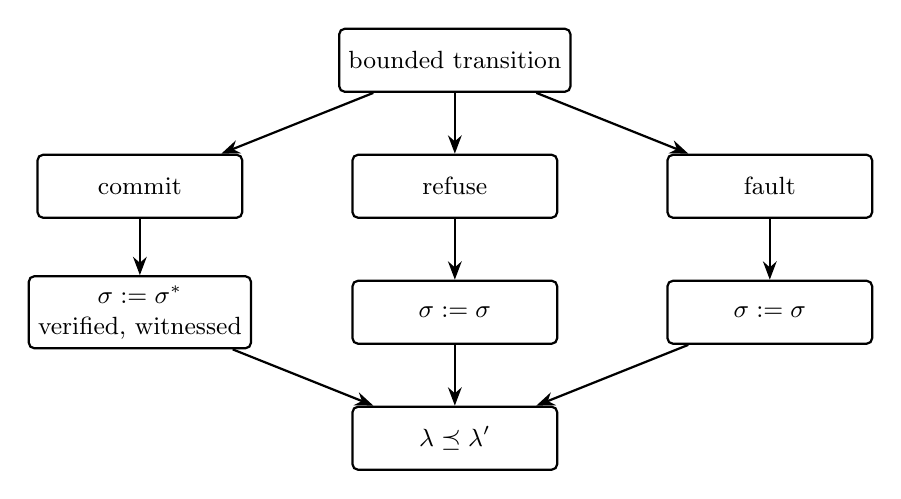
\begin{tikzpicture}[>=Stealth,thick,
  b/.style={draw,rounded corners=2pt,minimum width=2.6cm,minimum height=0.8cm,font=\small,align=center}]
\node[b] (t) at (4,3.2) {bounded transition};
\node[b] (c) at (0,1.6) {commit};
\node[b] (r) at (4,1.6) {refuse};
\node[b] (f) at (8,1.6) {fault};
\node[b] (cs) at (0,0) {$\sigma:=\sigma^{\ast}$\\ verified, witnessed};
\node[b] (rs) at (4,0) {$\sigma:=\sigma$};
\node[b] (fs) at (8,0) {$\sigma:=\sigma$};
\node[b] (l) at (4,-1.6) {$\lambda\pre\lambda'$};
\draw[->] (t) -- (c); \draw[->] (t) -- (r); \draw[->] (t) -- (f);
\draw[->] (c) -- (cs); \draw[->] (r) -- (rs); \draw[->] (f) -- (fs);
\draw[->] (cs) -- (l); \draw[->] (rs) -- (l); \draw[->] (fs) -- (l);
\end{tikzpicture}
\caption{Theorem~\ref{t:sound}: three outcomes, one prefix-preserved ledger.}
\end{figure}

\section{Negative Examples}\label{s:neg}

The ordering discipline is justified by programs that must be rejected. The following are ill-formed under the static judgment.

\begin{Verbatim}
<( req  ~ write  ? allowed  ! chk  @ src  > done )>
\end{Verbatim}
\emph{Admission after transformation.} In the core this is harmless, since \code{?} reads $\sigma_0$. In any extension where a transformer can produce an effect, the test would run after the effect and refusal could not preserve state. The static judgment excludes the pattern in the core so that extensions cannot introduce it silently.

\begin{Verbatim}
<( req  ? allowed  ~ write  @ src  > done  ! chk )>
\end{Verbatim}
\emph{Verification after commit.} The commit clause is not last. Verification cannot establish the invariant after the store has been installed, and Proposition~\ref{p:vc} fails for the resulting trace: the commit precedes any \textsf{ver} entry.

\begin{Verbatim}
<( req  ? allowed  ~ write  @ src  > done )>
\end{Verbatim}
\emph{No verification clause.} A commit reachable without verification would let a transition become durable on the strength of a pre-state test alone.

\begin{Verbatim}
<( req  ? allowed  ~ f  ! chk  @ src  > c1  > c2 )>
\end{Verbatim}
\emph{Two commits.} Exactly one commit clause is allowed, since Proposition~\ref{p:corr} counts one witness per commit and one commit per transition.

\section{Enclosing Boundaries}\label{s:bound}

A boundary is more than a grouping. If $B$ relates an outside and an inside, then for the boundary to be semantically real there must be a property $P$ with $P_{\mathrm{inside}}\neq P_{\mathrm{outside}}$. Applied to the core: the parenthesis \code{( )} marks an evaluation region, and fixes the order of reduction, but changes no admissibility, so it is a context and not a semantic boundary. The delimiters \code{<( )>} are a boundary in the strong sense, since inside a frame the visible store is $\sigma^{\ast}$ and outside it is $\sigma$. A boundary with no change in admissibility is representational decoration, and the criterion classifies the two pairs accordingly.

Crossing is asymmetric. Entering with a proposal and leaving with an outcome are not inverse operations, $\mathrm{exit}(\mathrm{enter}(v))\neq v$: what returns is a value, a refusal, or a fault, together with changes to state and ledger. The boundary is an operator on the conditions of return.

Consider an enclosing sequence of layers $1,\dots,n$, each contributing a guard applied to a proposed transition. Let $\mathcal T_0$ be the set of transitions a bounded transition may perform, and let $F_i$ be the operator by which layer $i$ modifies the permitted set:
\[
\mathcal T_{i}=F_i(\mathcal T_{i-1}).
\]
A boundary may transform transitions and not only accept or reject them. A purely restrictive layer satisfies $F_i(\mathcal T)\subseteq\mathcal T$.

\begin{proposition}[Restrictive boundaries narrow monotonically]\label{p:bound}
If every $F_i$ is restrictive, then $\mathcal T_n\subseteq\cdots\subseteq\mathcal T_1\subseteq\mathcal T_0$. If in addition each $F_i$ is a pointwise filter, $F_i(\mathcal T)=\mathcal T\cap A_i$, then $\mathcal T_n=\mathcal T_0\cap\bigcap_iA_i$.
\end{proposition}
\begin{proof}
The first claim is induction using $F_i(\mathcal T)\subseteq\mathcal T$. The second follows by unrolling the definition and using associativity and commutativity of intersection.
\end{proof}

The intersection formula is a special case that requires independence of the guards and a shared transition universe. Constraint composition need not be set intersection. Together with the terminality of refusal (Section~\ref{s:legal}) the result gives the formal counterpart of ``return outward carrying only what every enclosing boundary admits,'' in the case of restrictive layers. Figure~\ref{f:nest} shows the nesting.

\begin{figure}[h]
\centering
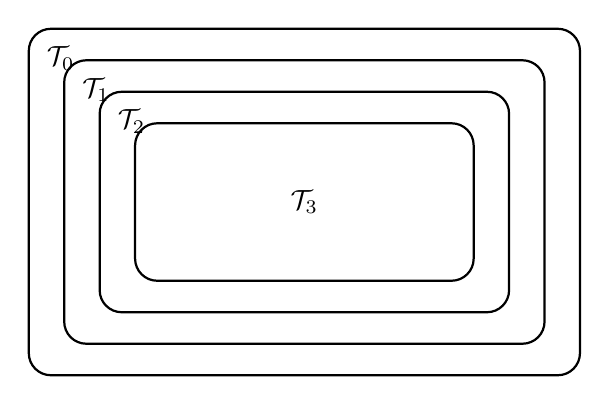
\begin{tikzpicture}[thick]
\draw[rounded corners=8pt] (0,0) rectangle (7,4.4);
\draw[rounded corners=8pt] (0.45,0.4) rectangle (6.55,4.0);
\draw[rounded corners=8pt] (0.9,0.8) rectangle (6.1,3.6);
\draw[rounded corners=8pt] (1.35,1.2) rectangle (5.65,3.2);
\node[anchor=north west] at (0.1,4.3) {$\mathcal T_0$};
\node[anchor=north west] at (0.55,3.9) {$\mathcal T_1$};
\node[anchor=north west] at (1.0,3.5) {$\mathcal T_2$};
\node at (3.5,2.2) {$\mathcal T_3$};
\end{tikzpicture}
\caption{Restrictive boundaries only: $\mathcal T_3\subseteq\mathcal T_2\subseteq\mathcal T_1\subseteq\mathcal T_0$. General boundaries may transform the set and are not drawn this way.}
\label{f:nest}
\end{figure}

\section{General Principles}\label{s:prin}

Several principles separate from the particular calculus and apply to any system with boundaries, proposals, and records.

\paragraph{Operational iconicity.} Syntax usually has conventional meaning. Here the design goal is that
\[
\mathrm{structure}(\text{representation})\approx\mathrm{structure}(\text{evaluation}).
\]
Nested regions correspond to nested evaluation, opening to entering, closing to returning, and sequential operators to successive motions. The relation is structure-preserving and not an identity between text and execution, and it is testable: the order of region entry in the trace must equal the pre-order of the AST (Section~\ref{s:proto}).

\paragraph{Witness feeds admissibility.} The event and the record of the event are different objects, $T\neq W(T)$, but the record can constrain later events, $W(T_t)\to A(T_{t+1})$. In the core the admission predicates do not read the ledger. An extension in which they do makes the admissible space a function of history,
\[
A_{t+1}=F(A_t,W_t),
\]
so that an event does not merely add a record but can change what may happen next. Prefix extension and legality are unaffected, since predicates remain pure.

\paragraph{Depth versus size.} A small expression can induce a long traversal. Run length in the core is bounded by program size, since there is no recursion, so the point applies to extensions and to the doorway analogy below: representations can be small because they preserve paths and not bodies.

\paragraph{Continuation over snapshot.} A witness stores $(t,\hash(\sigma_0),\hash(\sigma_1),V,A)$, that is, an edge and its authorization, and not a copy of either store. Figure~\ref{f:cont} contrasts what is preserved. To preserve a process it suffices to preserve enough to continue it, and not necessarily enough to copy it.

\begin{figure}[h]
\centering
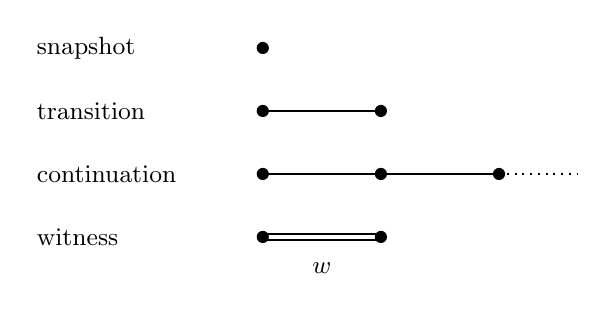
\begin{tikzpicture}[thick,every node/.style={font=\small}]
\node[anchor=west] at (0,2.4) {snapshot};
\fill (3,2.4) circle (2.2pt);
\node[anchor=west] at (0,1.6) {transition};
\fill (3,1.6) circle (2.2pt); \fill (4.5,1.6) circle (2.2pt); \draw (3,1.6)--(4.5,1.6);
\node[anchor=west] at (0,0.8) {continuation};
\fill (3,0.8) circle (2.2pt); \fill (4.5,0.8) circle (2.2pt); \fill (6,0.8) circle (2.2pt);
\draw (3,0.8)--(4.5,0.8)--(6,0.8); \draw[dotted] (6,0.8)--(7,0.8);
\node[anchor=west] at (0,0) {witness};
\fill (3,0) circle (2.2pt); \fill (4.5,0) circle (2.2pt);
\draw (3,0.04)--(4.5,0.04); \draw (3,-0.04)--(4.5,-0.04);
\node at (3.75,-0.4) {$w$};
\end{tikzpicture}
\caption{Preservation targets: a vertex, an edge, a path, and an edge together with its record.}
\label{f:cont}
\end{figure}

\section{Representation as Doorway}\label{s:door}

A concrete illustration is a 52-character string that encodes a video link. It is offered as an analogy, not as evidence for the semantics. The bytes do not contain the video. The URL does not contain the video. Even a time parameter such as \code{t=86} does not contain the event at that timestamp. The string preserves a traversable specification:
\[
b\xrightarrow{\ \mathrm{decode}\ }s\xrightarrow{\ \mathrm{parse}\ }r\xrightarrow{\ \mathrm{resolve}\ }_{\mathcal E}\,x.
\]
Each layer admits only certain transformations. Changing one byte may invalidate the string, whereas changing \code{86} to \code{87} preserves the resource and changes the requested coordinate. The important property is partiality:
\[
r\neq x,\qquad \mathrm{resolve}(r,\mathcal E)\rightharpoonup x.
\]
A doorway can fail to resolve (Figure~\ref{f:door}), which strengthens the analogy: a representation is a preserved possibility of traversal and not a guarantee of arrival. The witness of Section~\ref{s:corr} is the corresponding artifact for a state transition: it does not contain the transition but preserves enough structure for another evaluator to check it.

Three preservation targets are distinguished:
\[
\begin{array}{rcl}
\text{object preservation} &:& x_t=x_0,\\
\text{representation preservation} &:& r_t=r_0,\\
\text{reachability preservation} &:& \mathrm{resolve}(r_t,\mathcal E_t)\rightharpoonup x_t.
\end{array}
\]
The third is the interesting case: something can change substantially while remaining reachable through a valid continuation, and persistence of access is not persistence of object.

\begin{figure}[h]
\centering
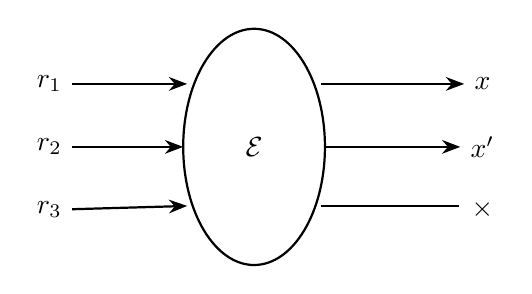
\begin{tikzpicture}[>=Stealth,thick]
\node (r1) at (0,1.6) {$r_1$}; \node (r2) at (0,0.8) {$r_2$}; \node (r3) at (0,0) {$r_3$};
\draw (2.6,0.8) ellipse (0.9 and 1.5); \node at (2.6,0.8) {$\mathcal E$};
\node (x1) at (5.5,1.6) {$x$}; \node (x2) at (5.5,0.8) {$x'$}; \node (x3) at (5.5,0) {$\times$};
\draw[->] (r1) -- (1.75,1.6); \draw[->] (3.45,1.6) -- (x1);
\draw[->] (r2) -- (1.7,0.8); \draw[->] (3.5,0.8) -- (x2);
\draw[->] (r3) -- (1.75,0.05); \draw (3.45,0.05) -- (5.2,0.05);
\end{tikzpicture}
\caption{Partial resolution. Two representations reach referents; the third does not resolve.}
\label{f:door}
\end{figure}

\section{Extensions Outside the Core}

The following are specified informally and are kept out of the proofs.

\paragraph{Persistence and reconstruction.} The flush motion \code{\#} binds the ledger to a host store. Durability guarantees, and the failure modes of an unavailable store, belong here, and an unavailable ledger is a fault, not a refusal. The reconstruct symbol \code{\^{}} recovers state from recorded continuations. The intended obligation is a non-invention property. If $R$ is an explicitly declared set of reconstruction rules and $\mathrm{Closure}(W,R)$ is what can be derived from witnessed records $W$ under $R$, then
\begin{gather*}
\mathrm{Recover}(W)\preceq\mathrm{Closure}(W,R),\\
\mathrm{Recover}(W)\not\models q\ \text{ whenever } q\text{ is not derivable from }W\text{ under }R.
\end{gather*}
Recovery may reconstruct what the evidence licenses and may not silently manufacture continuity. As stated this is close to a definition, so the substantive obligation falls on the implementation: to show that the recovery procedure is sound with respect to the closure.

\paragraph{Closed nesting and concurrency.} In the core a bounded transition placed in the proposal position of another is evaluated to completion, including its own commit, before the outer frame opens. It is a sequential composition. Closed nesting, in which an inner commit installs into the outer staged store, requires an additional rule, and concurrency requires a validation step at commit. Each introduces sources of nondeterminism that Proposition~\ref{p:det} excludes.

\paragraph{Larger interpretations.} Semantic interpretations of the calculus into other frameworks are treated as maps $\mathcal I:C\to\Phi$ out of the calculus. The proofs do not depend on any such framework, and a framework may consume the semantics without being presupposed by it.

\section{ASCII as a Representational Invariant}

The restriction to printable ASCII fixes a representational invariant, and not a semantic one. Replacing a symbol by a Unicode glyph need not change its denotation, and the essay does not claim otherwise. What the restriction secures is the round trip of Proposition~\ref{p:parse}: with a canonical layout, $\mathrm{print}(\mathrm{parse}(s))=s$, so the source that displays the structure and the bytes that store it are the same object, and the claim that the same source yields the same diagram becomes testable. A program survives terminals, shells, version-control diffs, serial links, minimal editors, and archival formats without a rendering layer. The proposition under test is that a spatially suggestive notation does not require a graphical interface: indentation and nesting of ASCII delimiters can carry the structural information of a diagram if the operators are chosen so that layout and evaluation order agree.

\section{Prototype and Evaluation Criteria}\label{s:proto}

A reference interpreter follows the levels of Section~\ref{s:core}. It tokenizes the reserved symbols, parses into well-formed ASTs, rejects ill-formed programs with a specific reason, executes the small-step rules, and emits a trace. Trace entries carry region identifiers,
\[
t_i=(\mathit{region},\,\mathit{operation},\,\mathit{input},\,\mathit{result}),
\]
since without them different programs could produce identical traces. The interpreter should be small enough to read in one sitting.

The language is not evaluated by asserting that it is better. Each result of the paper is a property that can be tested mechanically on generated and hand-written programs, in the manner of property-based testing, so that the prototype functions as an executable test of the formal claims and not as an illustration of them.

\begin{enumerate}[label=(\roman*)]
\item \textbf{Round trip.} $\mathrm{print}(\mathrm{parse}(s))=s$ on canonical sources (Prop.~\ref{p:parse}).
\item \textbf{Determinism.} Repeated runs from the same configuration produce identical traces (Prop.~\ref{p:det}).
\item \textbf{Iconicity.} The order of region entry and exit in the trace matches the order derived from the AST. The trace determines the sequence of region entries and exits, and full source reconstruction is not claimed (Prop.~\ref{p:trav}).
\item \textbf{Isolation.} $\sigma$ and $\omega$ are constant between an open step and the corresponding commit, tested with transformers that would emit effects if permitted (Prop.~\ref{p:loc}).
\item \textbf{Legality.} Every ledger belongs to the prefix language of Proposition~\ref{p:legal}, checked by a small automaton.
\item \textbf{Inert refusal and fault.} On every refused or faulted transition, $\sigma$ and $\omega$ are unchanged (Prop.~\ref{p:ref}).
\item \textbf{Verified commit and correspondence.} A trace checker computes $\mathrm{ValidWitness}$ from the trace alone and confirms Propositions~\ref{p:vc} and~\ref{p:corr}, including count equality at every prefix.
\item \textbf{Negative cases.} Each program of Section~\ref{s:neg} is rejected for the stated reason, and a variant interpreter that admits it exhibits the predicted failure.
\item \textbf{Motion table.} Each transition rule belongs to exactly one motion and each core motion has a symbol (Section~3).
\end{enumerate}
A failed check is informative. If (iii) fails the layout does not mirror evaluation for that construct. If (ix) fails, some symbol is doing more than one job or some motion is unnamed, and the design principle has been violated.

\section{Non-Collapse Principles}\label{s:noncollapse}

The results above can be summarized as a family of distinctions. Each is instantiated at a specific point of the calculus, and none is an imposed philosophical claim.

\begin{table}[h]
\centering
\small
\begin{tabular}{@{}p{0.32\linewidth}p{0.6\linewidth}@{}}
\toprule
Distinction & Where it is instantiated \\
\midrule
representation $\neq$ referent & partial resolution; parse versus evaluate (Sections~2, 13) \\
proposal $\neq$ realization & $\mathcal R\subseteq\mathcal E\subseteq\mathcal P$; refusal preservation (Prop.~\ref{p:ref}) \\
evaluation $\neq$ exposure & staged store; boundary locality (Prop.~\ref{p:loc}) \\
admission $\neq$ verification & signatures of \code{?} and \code{!}; prospective versus relational (Section~3) \\
event $\neq$ witness & recorded versus valid; $w\neq T$ (Section~\ref{s:corr}) \\
refusal $\neq$ absence & $\Delta\sigma=0$ with $\Delta\lambda\neq0$ (Prop.~\ref{p:ref}) \\
persistence $\neq$ truth & valid witness certifies structure, not content (Section~\ref{s:corr}) \\
recovery $\neq$ invention & closure bound on reconstruction (Section~14) \\
\bottomrule
\end{tabular}
\caption{Non-collapse principles and their instances.}
\end{table}

The calculus works by refusing to collapse objects that ordinary description casually identifies. Evaluation proceeds inward by decomposition, and continuation proceeds outward by admissibility. The ASCII language is an economical demonstration of that thesis and is not the thesis itself. The essay is about the relations among representation, traversal, boundary, admissibility, witness, and continuation, and the notation is the small formal object through which those relations become visible.

\section{Related Work and Claimed Contribution}

None of the following is claimed as new individually: symbolic domain-specific languages, visible evaluation structure, ASCII notations, transaction-like semantics, or Lisp-style nesting. Lisp and Scheme supply the identification of program text with tree structure~\cite{sicp}. Teaching notations that draw nested circles motivate the reading of parentheses as evaluation boundaries~\cite{bootstrap}. Concatenative languages such as Forth show that a very small symbolic vocabulary can carry substantial semantics~\cite{forth}. Evaluation contexts and syntactic operational semantics supply the machinery of Section~\ref{s:core}~\cite{felleisen,wright,plotkin}. Effect systems classify computations by the effects they may perform~\cite{gifford}, which is the natural home of the compensable and irrevocable distinction. The transactional properties are those of the database tradition~\cite{haerder} and of transactional memory~\cite{herlihy}. The ledger is close to event sourcing~\cite{fowler}, and the recorded-versus-valid distinction is close to work on provenance~\cite{buneman}. Capability-oriented design motivates restricting what a transformer may reach~\cite{miller}, and reversible computation~\cite{bennett} motivates the care taken over what recovery may claim.

The candidate contribution is the particular conjunction:
\begin{quote}
evaluation-visible ASCII syntax, plus bounded admissibility, plus witness-producing transitions, plus formal traversal semantics.
\end{quote}
Its value, if any, lies in the fact that each symbol is tied to a restriction on transitions, each restriction is tied to a proved property, and a small interpreter can check every such property.

\section{Limitations}

The core is sequential and deterministic, and the guarantees weaken when those assumptions are relaxed. The meta-level functions $p,f,q,g$ are assumed given, and their correctness is outside the calculus. The hash assumption is a modelling device. Validity of a witness concerns structure and does not extend to the truth of predicates beyond the fact that they returned true. The proofs are by inspection of the rules and have not been mechanized. The evaluation criteria test internal consistency and legibility. Whether programmers make fewer errors in this notation is a separate empirical question that would require a user study.

\section{Conclusion}

Parentheses expose the structure of evaluation. A small set of further symbols can be assigned distinct restrictions on state transition: admit against the pre-state, transform a staged store, verify the before-and-after relation, attribute provenance, and commit as the only durable write. With well-formedness fixing their order, the core calculus yields a chain of results: parsing is unique, the machine is deterministic, nested evaluation decomposes into inner and outer runs, staging isolates committed state, ledger histories are legal and only extend, refusal and fault change nothing but the ledger, commit implies verification, commits correspond to valid witnesses, and restrictive boundaries only narrow what may pass. The chain closes in a single soundness theorem for bounded transitions. Beneath it lies a second chain of distinctions the calculus declines to collapse. The evocative language survives as commentary on these results and does not stand in for them.

\begin{thebibliography}{99}
\bibitem{sicp} H.~Abelson and G.~J.~Sussman, \emph{Structure and Interpretation of Computer Programs}, 2nd ed., MIT Press, 1996.
\bibitem{bootstrap} E.~Schanzer, K.~Fisler, S.~Krishnamurthi, and M.~Felleisen, ``Transferring skills at solving word problems from computing to algebra through Bootstrap,'' \emph{Proc.\ SIGCSE}, 2015.
\bibitem{forth} L.~Brodie, \emph{Starting Forth}, Prentice Hall, 1981.
\bibitem{felleisen} M.~Felleisen and R.~Hieb, ``The revised report on the syntactic theories of sequential control and state,'' \emph{Theoretical Computer Science} 103(2), 1992.
\bibitem{wright} A.~K.~Wright and M.~Felleisen, ``A syntactic approach to type soundness,'' \emph{Information and Computation} 115(1), 1994.
\bibitem{plotkin} G.~D.~Plotkin, ``A structural approach to operational semantics,'' \emph{Journal of Logic and Algebraic Programming} 60--61, 2004.
\bibitem{gifford} D.~K.~Gifford and J.~M.~Lucassen, ``Integrating functional and imperative programming,'' \emph{Proc.\ ACM Conference on LISP and Functional Programming}, 1986.
\bibitem{haerder} T.~Haerder and A.~Reuter, ``Principles of transaction-oriented database recovery,'' \emph{ACM Computing Surveys} 15(4), 1983.
\bibitem{herlihy} M.~Herlihy and J.~E.~B.~Moss, ``Transactional memory: architectural support for lock-free data structures,'' \emph{Proc.\ ISCA}, 1993.
\bibitem{fowler} M.~Fowler, ``Event sourcing,'' online article, 2005.
\bibitem{buneman} P.~Buneman, S.~Khanna, and W.-C.~Tan, ``Why and where: a characterization of data provenance,'' \emph{Proc.\ ICDT}, 2001.
\bibitem{miller} M.~S.~Miller, \emph{Robust Composition: Towards a Unified Approach to Access Control and Concurrency Control}, PhD thesis, Johns Hopkins University, 2006.
\bibitem{bennett} C.~H.~Bennett, ``Logical reversibility of computation,'' \emph{IBM Journal of Research and Development} 17(6), 1973.
\end{thebibliography}

\end{document}
